\subsubsection{Tổng quan các dịch vụ của hệ thống}

\begin{figure}[H]
\centering
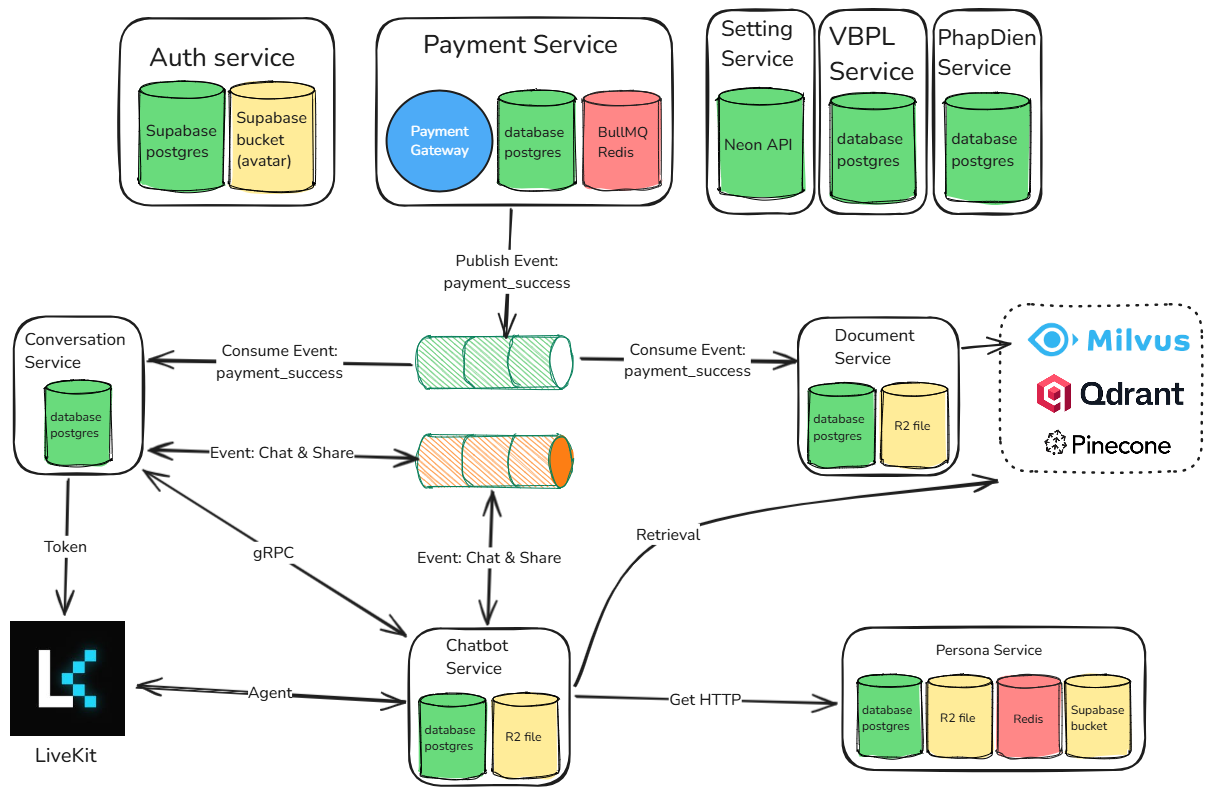
\includegraphics[width=0.85\textwidth]{pictures/Microservice-all.excalidraw.png}
\caption{Sơ đồ tổng quan các dịch vụ của hệ thống}
\end{figure}

Tất cả các dịch vụ đều dùng supabase
để xác thực thông tin JWT của người dùng.
Trong JWT có các thông tin sub, exp, email, aal, app\_metadata, \dots.
Các dịch vụ giải mã để lấy thông tin người dùng.
Kết quả thông tin payload của JWT từ Supabase:

\begin{figure}[H]
\centering
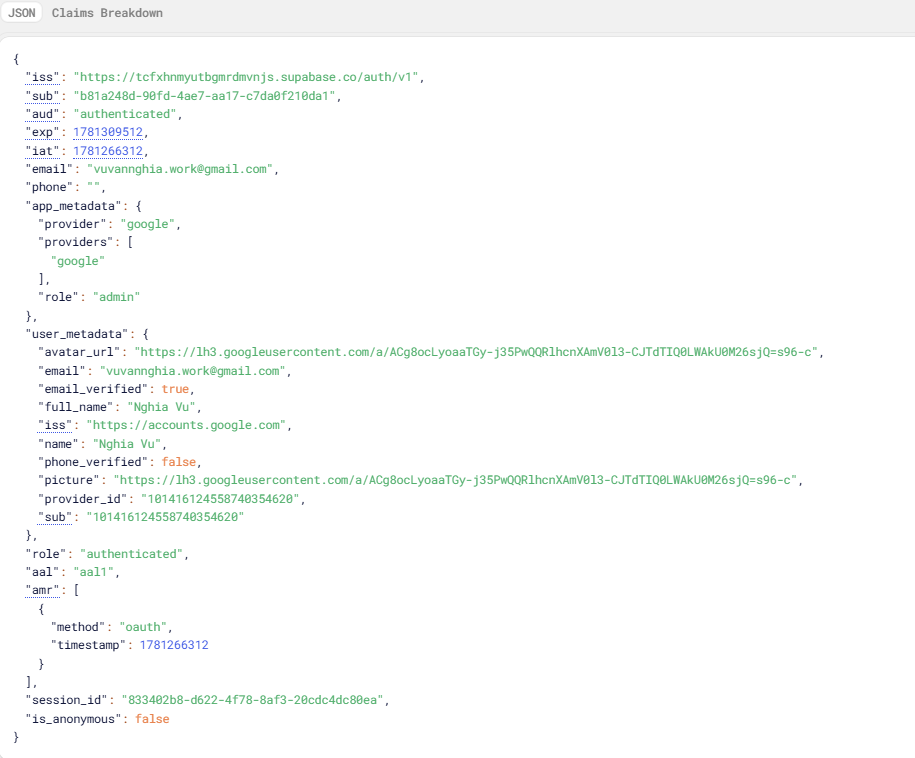
\includegraphics[width=0.85\textwidth]{pictures/auth-jwt-supabase.png}
\caption{Thông tin JWT Payload từ Supabase}
\end{figure}

\textbf{Thuật toán TOTP (Time-based One-time Password)}
sử dụng yếu tố thời gian Unix
(thay vì dùng bộ đếm)
(thời gian $T_0$ của Unix là ngày 1 tháng 1 năm 1970).
Giá trị của bộ đếm trong thuật toán TOTP được tính bằng công thức:

\[C_T = \left[\frac{T-T_0}{T_X}\right]\]

Trong đó:

\begin{itemize}
\item $T$ là thời gian hiện tại
\item $T_0$ là thời gian đầu tiên
\item $T_X$ là chu kỳ của mã TOTP (mặc định là 30 giây)
\end{itemize}

Sau khi thực hiện xong thuật toán TOTP,
lần đầu tiên máy chủ cần trao đổi khóa bí mật với người dùng.
Vì hiện nay điện thoại thông minh đều được trang bị camera,
máy chủ có thể chuyển đổi khóa bí mật thành mã QR
và yêu cầu người dùng phần mềm Authenticator
quét mã QR để lấy khóa bí mật.

\begin{figure}[H]
\centering
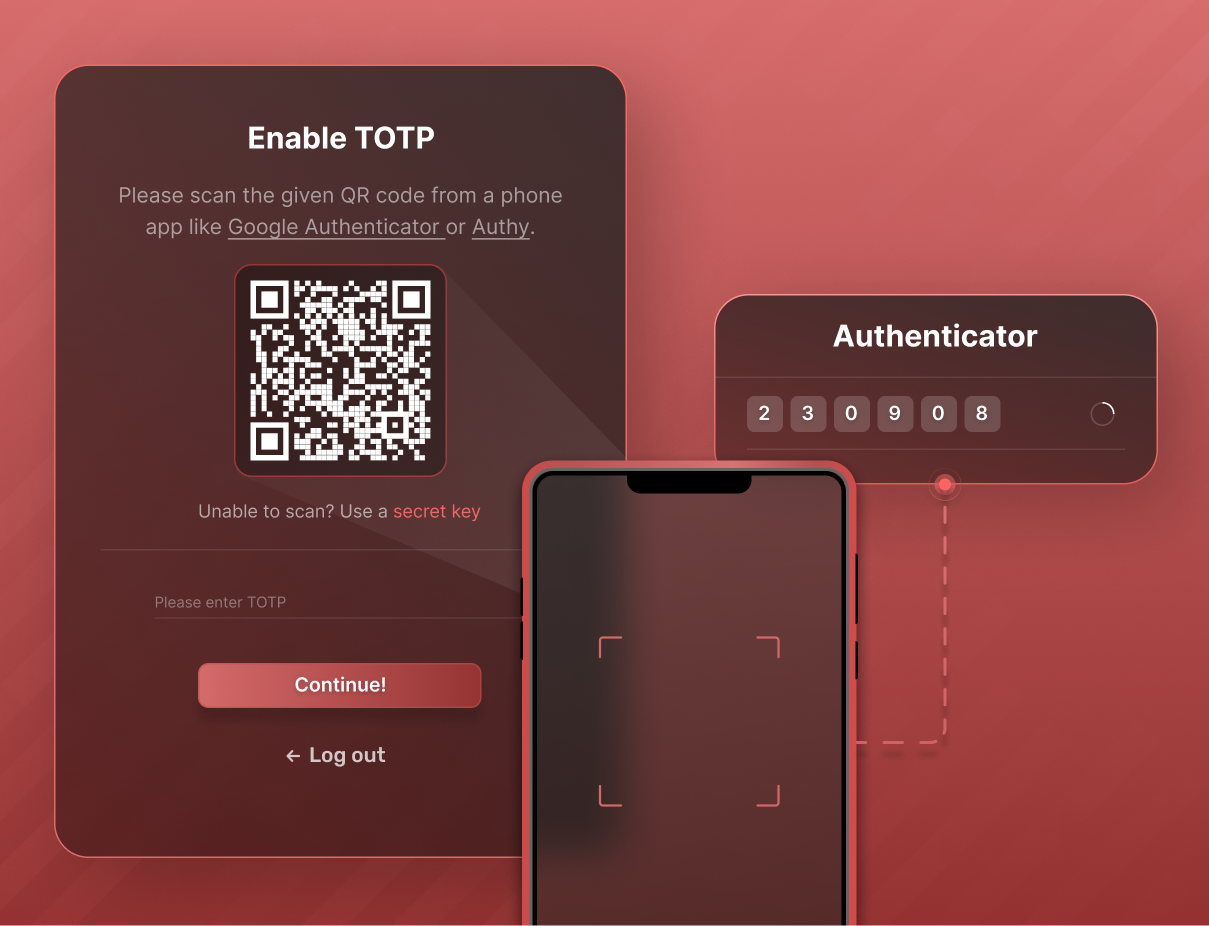
\includegraphics[width=0.6\textwidth]{pictures/why-totp.png}
\caption{Trao đổi khóa bí mật bằng cách quét mã QR}
\end{figure}

TOTP sử dụng khóa bí mật có thể hiển thị dưới dạng mã QR cho người dùng.
Từ đó, máy chủ và phần mềm Authenticator đều có thể tính được giá trị của
mã TOTP theo thuật toán.
Cuối cùng, khi cần xác thực thì người dùng nhập giá trị TOTP
hiển thị trên phần mềm Authenticator để máy chủ tiến hành so sánh.

\begin{figure}[H]
\centering
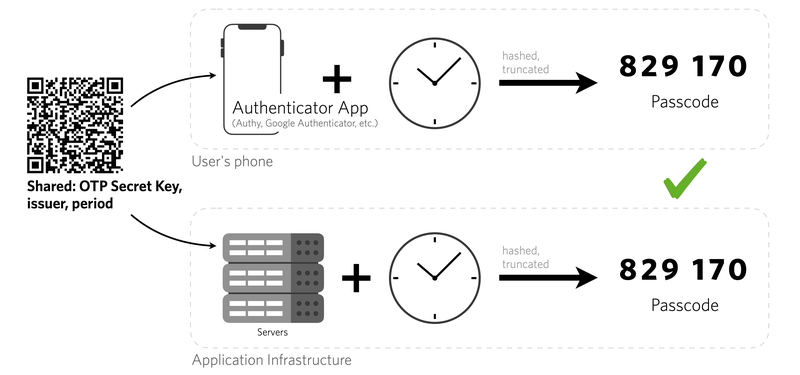
\includegraphics[width=0.95\textwidth]{pictures/2fa_diagram.jpg}
\caption[Cách hoạt động của TOTP]{Cách hoạt động của TOTP (Nguồn: \cite{twilio-totp})}
\end{figure}

Tham khảo tài liệu tại:
\url{https://supabase.com/docs/guides/auth/auth-mfa/totp}.
% của Supabase.
Trang tài liệu này của Supabase
hướng dẫn cách triển khai
tính năng xác thực đa yếu tố (MFA) bằng ứng dụng Authenticator (TOTP).
% trong Supabase.
Tính năng này hiện được cung cấp miễn phí
và bật mặc định cho mọi dự án Supabase.
Nội dung chính xoay quanh hai luồng hoạt động cơ bản:

\mbox{}\\
\textbf{Quy trình đăng ký yếu tố bảo mật (Enrollment Flow)}
\begin{enumerate}
\item Khởi tạo quá trình đăng ký.
\item Hệ thống sẽ trả về một mã QR và một chuỗi mã bí mật.
\item Người dùng sẽ dùng ứng dụng xác thực (như Google Authenticator) để quét mã QR này.
\item Chuẩn bị hệ thống để tiếp nhận mã xác minh, đồng thời trả về một challenge ID.
\item Đối chiếu mã 6 chữ số mà người dùng nhập vào từ ứng dụng xác thực.
\item Nếu mã hợp lệ, yếu tố bảo mật MFA này sẽ chính thức được kích hoạt cho tài khoản.
\end{enumerate}

\mbox{}\\
\textbf{Quy trình kiểm tra khi đăng nhập (Challenge Flow)}
\begin{enumerate}
\item Trích xuất danh sách các yếu tố MFA đã được người dùng đăng ký để lấy \texttt{factorId}.
\item Khi đã có \texttt{factorId}, ứng dụng tiếp tục gọi \texttt{challenge()} để mở phiên thử thách.
\item Dùng \texttt{verify()} cùng với mã TOTP người dùng nhập vào để hoàn tất đăng nhập và nâng cấp phiên làm việc lên \texttt{aal2}.
\end{enumerate}

\begin{figure}[H]
\centering
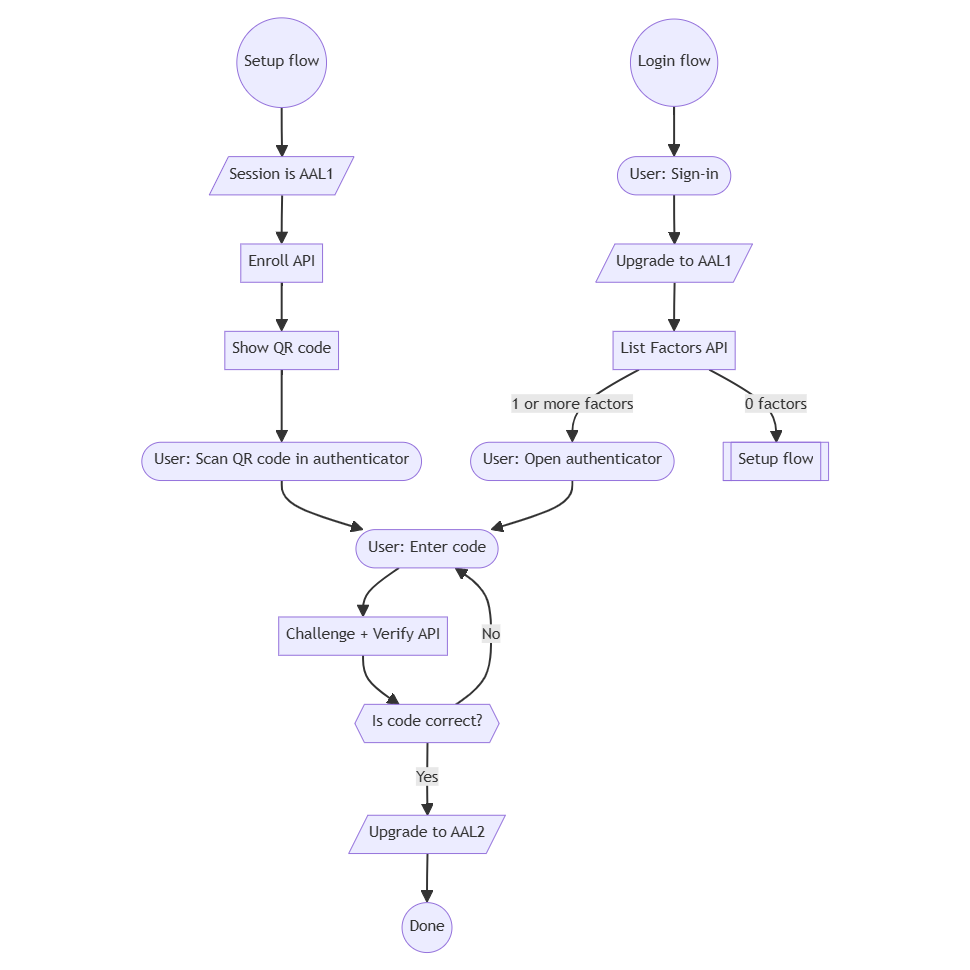
\includegraphics[width=0.95\textwidth]{pictures/auth-mfa-flow.excalidraw.png}
\caption[Sơ đồ luồng xử lý xác thực MFA Supabase]{Sơ đồ luồng xử lý xác thực MFA Supabase (Nguồn: \cite{supabase-totp})}
\end{figure}

Tất cả các dịch vụ đều dùng CSDL Postgres của Neon để làm CSDL riêng theo đúng mẫu CSDL cho mỗi dịch vụ (database per service pattern). Mỗi dịch vụ sẽ sở hữu và quản lý hoàn toàn CSDL của riêng nó.

\begin{figure}[H]
\centering
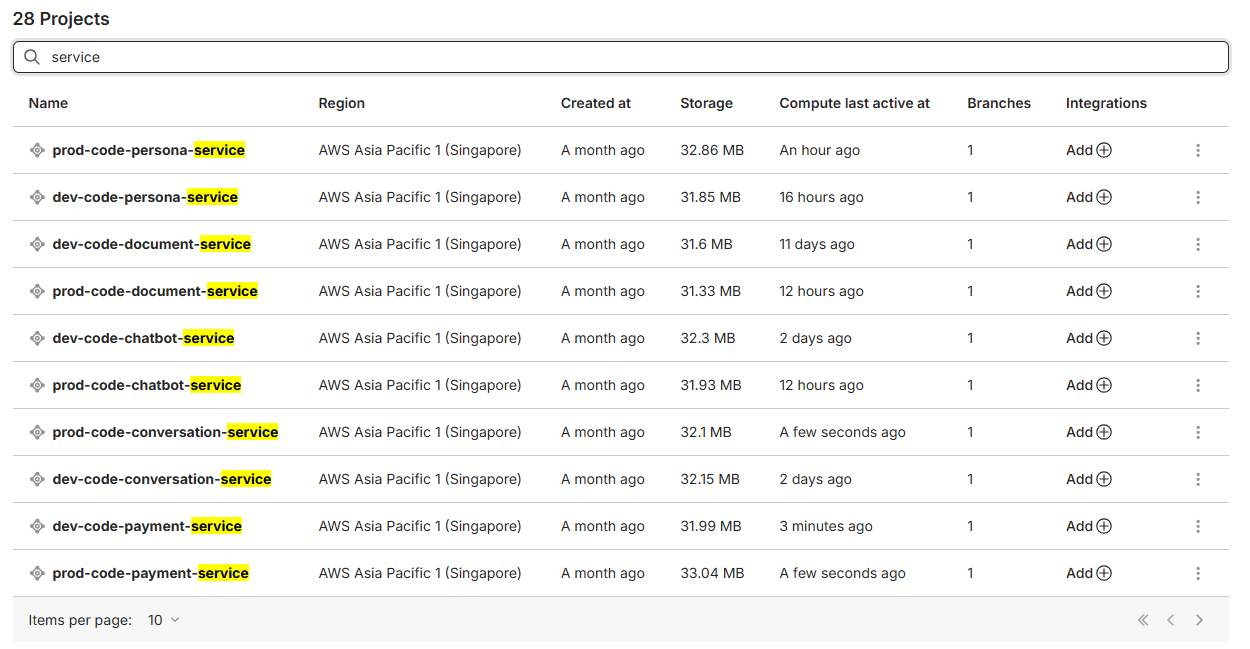
\includegraphics[width=0.8\textwidth]{pictures/neon-database-all.png}
\caption{Bảng điều khiển CSDL trong Neon}
\end{figure}

Các dịch vụ ngoại trừ auth service
và setting service được cấu hình
trong Kong API Gateway đơn giản
chỉ cần tạo Service và Route để định tuyến yêu cầu.
Dịch vụ auth service và setting service sẽ được mô tả chi tiết
về cách cấu hình Kong API Gateway
trong nội dung trình bày của chính dịch vụ đó.
Vì trang thống kê thông tin
đường ống dữ liệu (Data Pipeline)
dành cho quản trị viên (ADMIN)
có tần suất truy vấn thấp
nên sẽ được triển khai trên Vercel.

\begin{figure}[H]
\centering
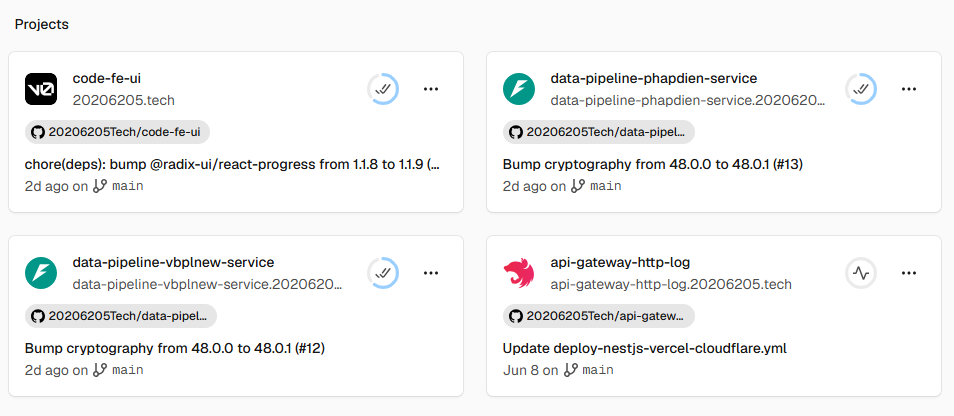
\includegraphics[width=0.95\textwidth]{pictures/vercel-project.png}
\caption{Bảng điều khiển các dự án trên Vercel}
\end{figure}

Các dịch vụ NestJS sử dụng Codecov để theo dõi độ bao phủ kiểm thử (test coverage).

\begin{figure}[H]
\centering
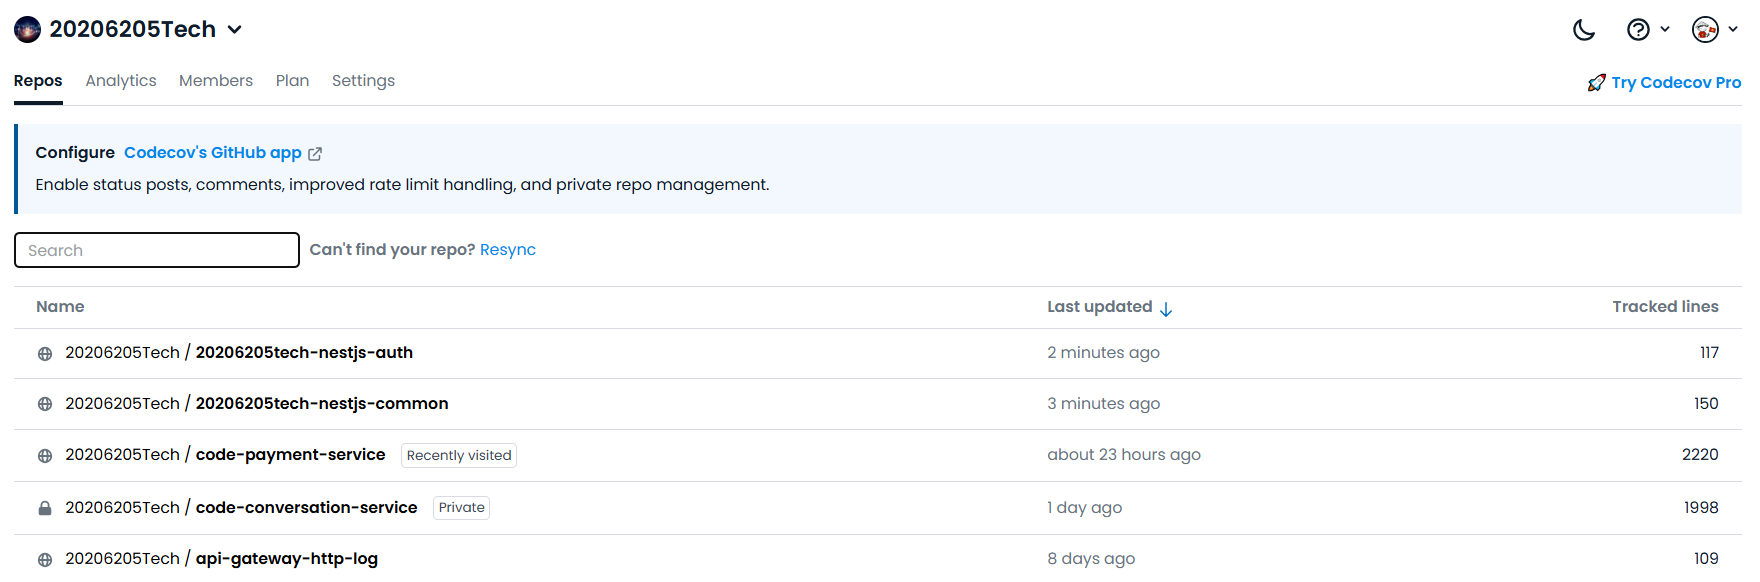
\includegraphics[width=0.95\textwidth]{pictures/test-codecov2.png}
\caption{Sử dụng CodeCov theo dõi độ bao phủ kiểm thử}
\end{figure}

Tích hợp SonarQube để phân tích chất lượng mã nguồn và các lỗ hổng bảo mật.

\begin{figure}[H]
\centering
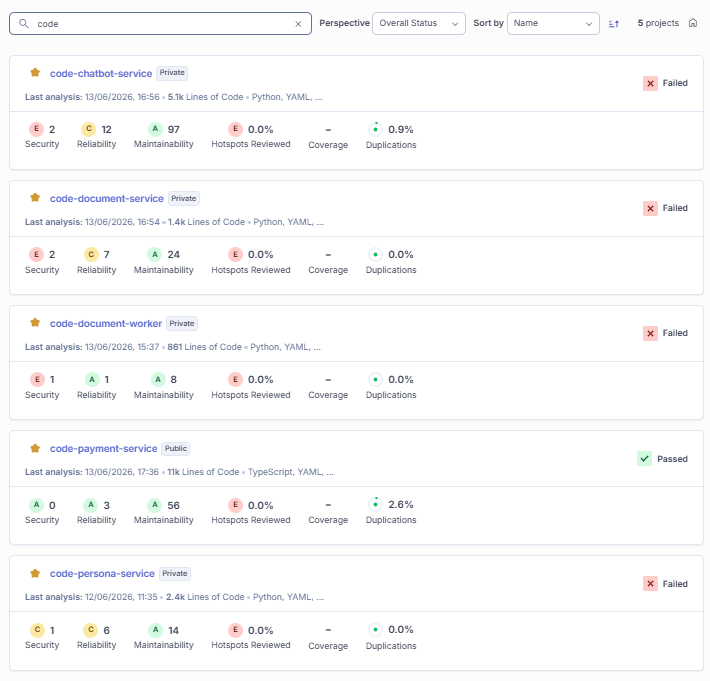
\includegraphics[width=0.8\textwidth]{pictures/sonarqube.png}
\caption{Giao diện phân tích mã nguồn trên SonarQube}
\end{figure}

% \subsubsection{Tracing và Quan sát hệ thống (Observability)}
% Hệ thống sử dụng \textbf{OpenTelemetry (OTel)} tích hợp trong tất cả các dịch vụ để tự động thu thập dấu vết phân tán (distributed traces) và gửi dữ liệu về Honeycomb.
Hệ thống
tích hợp Honeycomb để theo dõi vết
(distributed tracing) giữa các dịch vụ.

\begin{figure}[H]
\centering
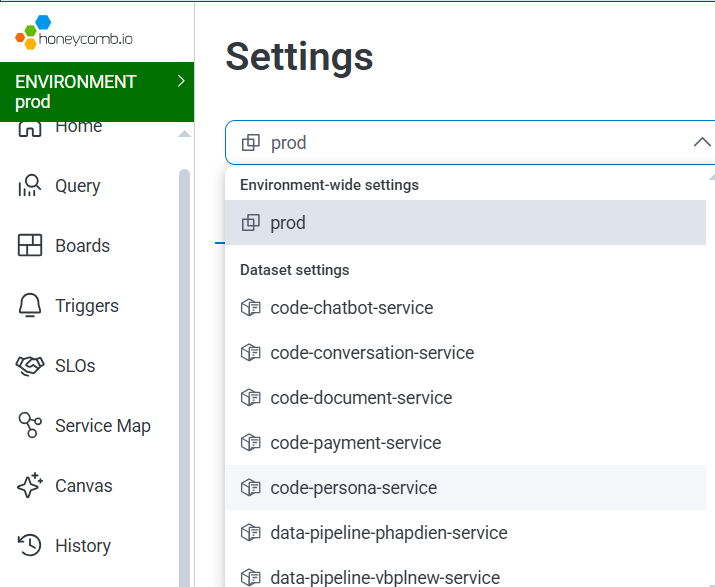
\includegraphics[width=0.7\textwidth]{pictures/tracing.png}
\caption{Giao diện theo dõi vết distributed tracing trên Honeycomb}
\end{figure}
